% ch02: 原文 GLDraft_D.tex 行 291–559；§2.1–2.2
% 只译散文（标题、正文、图题、脚注）；公式、\label、\ref、\eqref、\cite、图文件名保持不变。

\section{基本设置}\label{basic}

本节解释我们研究几何朗兰兹解析版本所用的基本框架，并回顾部分背景。

\subsection{通过膜量子化}\label{background}

这里我们简要概述若干在别处已有更完整论述的内容 \cite{GuW,GW}。我们先解释通过膜实现的形变量子化，然后说明量子化。

设 $Y$ 是复辛流形，复结构为 $I$，全纯辛形式为 $\Omega$。我们把 $Y$ 看作实辛流形，其辛形式为 $\omega_Y=\Im\,\Omega$。我们假定 $Y$ 使得以 $Y$ 为靶空间的量子 $\sigma$-模型存在（作为紫外完备的量子场论），并考虑按标准方式扭化该 $\sigma$-模型所得的 $A$-模型。一般并不知道对哪一类 $Y$ 该 $\sigma$-模型确实存在，但人们相信一个充分条件是：$Y$ 的复辛结构可延拓为完备的超凯勒（hyperkähler）结构。本文所看重的例子是 $Y$ 为希格斯丛模空间 $\M_H$ 的情形——它确实容许完备的超凯勒度量 \cite{H}——或为乘积 $\M_H\times \M_H$（两个因子上取相反的复结构、复共轭的辛结构），后者当然也有完备的超凯勒度量。

一般地，辛流形 $Y$ 的 $A$-模型除了通常的拉格朗日膜（其支撑为 $Y$ 的中维子流形）之外，还可以有余迷向膜（coisotropic brane），支撑在 $Y$ 的一个高于中维的余迷向子流形上 \cite{KO}。\zy{余迷向膜是支撑维数高于中维的 $A$-膜；当它支撑整个 $Y$、且 $\CP$ 丛曲率满足 $\I=\omega^{-1}(\sF+\sB)$ 为可积复结构时，就给出本文所用的秩 1 例子（Kapustin–Orlov 条件）。参见 \cite{KO}。} 最简单、也是本文唯一需要的情形，是支撑为整个 $Y$ 的秩 1 余迷向 $A$-膜。设 $\sB$ 是该 $\sigma$-模型的 $B$-场，考虑一个支撑为 $Y$ 的膜，其 Chan–Paton 丛（或 $\CP$ 丛）是线丛 $\L\to Y$，并带曲率为 $\sF=\d\sA$ 的酉联络 $\sA$。这组数据要定义一个 $A$-膜，其 Kapustin–Orlov 条件是 $\I=\omega_Y^{-1}(\sF+\sB)$ 应为 $Y$ 上可积的复结构。这个条件立即给出两个解。一个选择是 $\sF+\sB=\Re\,\Omega$，$\I=I$。由此构造的膜，我们称之为典范余迷向 $A$-膜（canonical coisotropic A-brane），记作 $\B_\cc$。第二个选择是 $\sF+\sB=-\Re\,\Omega$，$\I=-I$。这给出我们所谓的共轭典范余迷向 $A$-膜，记作 $\bB_\cc$。为对称地处理这两种情形，本文中方便的做法是取\footnote{这一选择是 \cite{GuW} 中作出的。不过，当只涉及 $\B_\cc$、$\bB_\cc$ 之一时，取 $\sF=0$、$\sB=\Re\,\Omega$ 可能更简单。} $\sB=0$，$\sF=\pm \Re\,\Omega$。这个选择只有在存在曲率为 $\Re\,\Omega$ 的复线丛 $\L\to Y$ 时才可能。在我们对希格斯丛模空间的应用中，$\Re\,\Omega$ 在上同调意义下平凡，故 $\L$ 存在，并可假定为拓扑平凡。

现在考虑代数 $\A=\Hom(\B_\cc,\B_\cc)$（按物理的说法，它是 $(\B_\cc,\B_\cc)$ 开弦的空间，其结合乘法来自开弦的拼接）。设 $\Omega=\Omega_0/\hbar$，其中 $\Omega_0$ 固定，$\hbar$ 变动。当 $\hbar\to 0$ 时，$\A$ 退化为 $Y$ 在复结构 $I$ 下全纯函数的交换代数 $\A_0$。在 $\hbar$ 阶上，$\A$ 中的乘法律与 $\A_0$ 中的交换乘法律相差一个由 泊松括号 $\{f,g\}=(\Omega^{-1})^{ij}\partial_i f\partial_j g$ 给出的项。因此 $\A$ 可看作 $\A_0$ 的形变量子化。$\bA=\Hom(\bB_\cc,\bB_\cc)$ 以同样方式联系于 $Y$ 在复结构 $-I$ 下全纯函数（等价地说，复结构 $I$ 下反全纯函数）的交换代数 $\bA_0$，并可看作 $\bA_0$ 的形变量子化。

一般而言，形变量子化是一种形式程序，必须在 $\hbar$ 的形式幂级数环上定义。当 $Y$ 的量子 $\sigma$-模型存在时，人们预期 $\hbar$ 可以取复数值（例如 1），而不必当作形式幂级数变量。在目前的例子中，可以对这一点给出更直接的解释。希格斯丛模空间 $\M_H(G,C)$ 具有 $\C^*$ 对称性，把希格斯场按 $\varphi\to \lambda\varphi$、$\lambda\in \C^*$ 重标度。这一操作以同样方式重标度 $\Omega$。当然，这只有在 $\Omega$ 于上同调意义下平凡时才可能。环 $\A_0$ 由按确定次数标度的函数（即 Hitchin 哈密顿量）生成，而标度对称性意味着形变环 $\A$ 中的所有关系都是形变参数 $\hbar$ 的多项式。因此取 $\hbar=1$ 有意义。当我们考虑量子化而非形变量子化时，类似的评论也适用，因为所考虑的重要膜都是 $\C^*$-不变的：标度对称性将意味着某些半经典公式实际上是精确的。

若 $Y$ 是仿射簇、拥有大量全纯函数，则形变量子化特别有意思。如前所述，在我们的主要例子中，$Y$ 将是 $\M_H$ 或 $\M_H\times \M_H$。$\M_H$ 远非仿射簇。当 $Y=\M_H$ 时，环 $\A_0$ 就是 Hitchin 纤维化底空间上的函数环；换言之，$\M_H$ 上的整体全纯函数就是 Hitchin 的 泊松交换哈密顿量的函数。Hitchin 的 泊松交换哈密顿量可以量子化为交换微分算子，作用在线丛 $K^{1/2}$ 的截面上，其中 $K$ 是 $\M_H$ 的典范丛。这一点由 Hitchin \cite{H2} 对 $G=\SU(2)$ 证明，并由 Beilinson 与 Drinfeld \cite{BD} 在一般情形证明。特别地，环 $\A$ 是交换的。泊松交换的经典哈密顿量可以量子化为交换微分算子这一事实，也可以用规范场论的语言看出，我们将在第 \ref{hh} 节与附录 \ref{coho} 中讨论。对于 $Y=\M_H\times\M_H$，形变量子化不过给出这一答案与其复共轭的乘积。

本文真正关心的是量子化，而非形变量子化。如何修改刚才描述的故事以包含量子化，已在 \cite{GuW,GW} 中解释。设 $M$ 是实辛流形，辛形式为 $\omega_M$，我们希望量子化它。（在我们的主要应用中，$M$ 将是 $\M_H$，视为实辛流形，而 $Y$ 将是 $\M_H\times \M_H$。）若 $M$ 有一个满足某些条件的复化 $Y$，则 $M$ 的量子化是 $Y$ 的 $A$-模型的一部分。$Y$ 应是复辛流形，其全纯辛形式 $\Omega$ 限制到 $M$ 上等于 $\omega_M$。此外，$Y$ 应有一个反全纯对合\footnote{对合是平方为 1 的自同构。} $\tau$，使 $M$ 是其不动点集的一个分支。这些条件蕴含 $\tau^*\Omega=\bar\Omega$。对于 $Y=\M_H\times \M_H$ 这一例子，反全纯对合就是交换两个因子的映射。最后，$Y$ 的量子 $\sigma$-模型必须存在。在这些条件下，取几何量子化意义上的预量子线丛 ${\frL}\to M$，\footnote{辛流形 $M$（辛形式为 $\omega$）上的预量子线丛，是复线丛 $\frL\to M$ 带一个曲率为 $\omega$ 的酉联络。}，就确定了一个支撑在 $M$ 上的 $A$-膜 $\B$。（其细节取决于在满足条件 $\sF+\sB=\Re\,\Omega$ 以定义膜 $\B_\cc$ 时所作的选择。我们将在第 \ref{cm} 节具体说明。）以辛结构 $\omega_M$ 与预量子线丛 $\frL$ 量子化 $M$ 所得的希尔伯特空间，其 $A$-模型答案为 $\H=\Hom(\B,\B_\cc)$。$\H$ 上埃尔米特内积的定义在第 \ref{cm} 节描述。

$\H$ 总是 $\A=\Hom(\B_\cc,\B_\cc)$ 的模。这可以这样表述：$M$ 上那些能解析延拓为 $Y$ 上全纯函数的函数，被量子化为 $\H$ 上的算子。此外，在温和条件下，$M$ 与自身之间一个可解析延拓为 $Y$ 与自身之间全纯对应的对应\footnote{$M$ 与自身之间的对应，简单地说就是 $M_1\times M_2$ 的一个拉格朗日子流形，其中 $M_1$、$M_2$ 是 $M$ 的两份拷贝，分别带辛结构 $\omega_M$ 与 $-\omega_M$。$Y$ 与自身之间的全纯对应类似地定义。}，可以自然地量子化为 $\H$ 上的算子。在 $M=\M_H$ 这一主要例子中，环 $\A$ 会相对较小，由全纯与反全纯 Hitchin 哈密顿量的多项式组成。作为补偿，有大量的对应——Hecke 对应——提供 $\H$ 上的额外算子。量子化这些对应很简单，因为可以援引形变量子化讨论中用过的 $\C^*$ 标度对称性。

我们是在二维 $\sigma$-模型的语境中描述这些的，这对于相当一般的实辛流形 $M$ 的量子化是合适的。然而，在 $M$ 是黎曼曲面 $C$ 上规范群为 $G$ 的希格斯丛模空间 $\M_H(G,C)$ 这一特殊情形，还有四维图像可用，它能给出远为完整的理解。为此，出发点是四维的、规范群为 $G$ 的 $\N=4$ 超杨–米尔斯理论。人们限制到形如 $\Sigma\times C$ 的四维流形上，其中 $\Sigma$ 是任意二维流形，而 $C$ 保持固定。在低能下，假定 $G$ 的中心平凡，该四维规范场论对许多目的而言约化为 $\Sigma$ 上以 $\M_H(G,C)$ 为靶空间的超对称 $\sigma$-模型 \cite{BJSV,JWS}。对四维 $\N=4$ 理论的某种扭化产生一个拓扑场论\footnote{如脚注 \ref{partial} 所述，这实际上是一个部分拓扑场论。}；当我们特殊化到形如 $\Sigma\times C$ 的四维流形时，它约化为 $\Sigma$ 上以 $\M_H(G,C)$ 为靶空间的 $A$-模型。$\sigma$-模型的膜 $\B_\cc$ 在四维规范场论中来自一个边界条件，它是对规范场 Neumann 边界条件的简单变形，并以半 BPS（half-BPS）方式延拓到整个超多重态；参见 \cite{KW} 第 12.4 节。

$\B_\cc$ 边界条件的四维提升有一个有趣而重要的特点。尽管它是某个具有完整四维拓扑对称性的 $A$-模型中的膜，膜 $\B_\cc$ 的定义却依赖于 $C$ 的复结构的选择。变形 Neumann 边界条件是四维拓扑场论的一个\emph{全纯-拓扑}（holomorphic–topological）局部边界条件。\footnote{具体地说，该边界条件破坏了物理理论的部分体超对称。其后果是，一些在体内为 $Q$-恰当的平移生成元，在边界存在时不再 $Q$-恰当，因而该边界条件在四维意义下不是拓扑的。$\B_\cc$ 依赖于复结构选择的另一种解释很简单：$\B_\cc$ 是用 $\sF+\sB=\omega_J$ 定义的，而后者的定义依赖于 $C$ 的复结构。关于 $\M_H$ 上哪些结构依赖或不依赖复结构的选择，见第 \ref{cm} 节开头的说明。} 支撑在点 $p\in C$ 处的边界局部算符可以全纯地依赖于 $p$，尽管它们拓扑地依赖于剩下的那一个边界方向。每当我们讨论自己构造的四维提升时，这一点都很重要。虽然 $A$-模型具有完整的四维拓扑不变性，但在膜 $\B_\cc$ 存在时，只有二维拓扑不变性可用。例如，在证明 Hitchin 哈密顿量与 Hecke 算符的交换性时，我们只用到二维拓扑不变性。

若 $G$ 有非平凡中心 $\zZ(G)$，则关于约化为 $\sigma$-模型的断言须稍作修改。更精确的说法是：在 $C$ 上紧致化后，四维规范场论对许多目的而言约化为以 $\M_H(G,C)$ 为靶空间的 $\sigma$-模型与一个规范群为有限群 $\zZ(G)$（平凡地作用在 $\M_H(G,C)$ 上）的规范场论的乘积。在我们想计算 Hitchin 哈密顿量与 Hecke 算符的本征值之前，这个有限规范群不起作用，因此在后文大部分内容中不会提到它。

通过以 $\M_H(G,C)$ 为靶空间的 $\sigma$-模型（可能再添上有限规范群）作纯粹二维的描述，对许多目的都有用。但约化到二维会丢失信息，要完整说明对偶就需要四维图像。\footnote{更准确地说，对偶的完整表述可以在四维中给出。对偶的更充分解释来自六维中的某个出发点 \cite{WittenLecture}。} 在标准数学处理中，一个类似的陈述是：几何朗兰兹对偶必须用 $G_\C$-丛或 $G_\C^\vee$ 局部系统的“栈”（stack）来表述，而不能用有限维模空间来表述。\zy{栈（stack）是模空间的范畴化推广，除对象外还记录对象之间的同构。正文所说的标准表述，用 $C$ 上 $G_\C$-丛的栈与 $G^\vee_\C$ 局部系统的栈代替有限维模空间。栈的一般定义可参看 Stacks Project 与 nLab 条目“stack”；此处“用栈表述”还意味着要满足下降（descent）条件。} 这两个陈述之间有简单的关系。Atiyah 与 Bott \cite{AB} 证明，光滑 $G$-丛 $E\to C$ 上所有 $G$-值联络构成的空间，连同复化规范变换群的作用，给出了全纯 $G_\C$-丛的栈的一个模型。这是因为任何联络的 $(0,1)$ 部分给 $E$（更确切地说，其复化）一个复结构，使它成为 $C$ 上的全纯 $G_\C$ 丛。
$\Sigma\times C$ 上 $G$-丛上的规范场，特别地确定了 $C$ 上规范场的一个以 $\Sigma$ 为参数族的族。因此任何这样的联络都确定一个从 $\Sigma$ 到 $C$ 上 $G_\C$ 丛的栈的映射。于是 $\Sigma\times C$ 上的 $\N=4$ 超杨–米尔斯理论可以理解为一个 $\Sigma$ 上的超对称 $\sigma$-模型，其靶空间是 $C$ 上 $G_\C$ 丛的栈。（在这个表述中，该理论是 $\Sigma$ 上的二维超对称规范场论耦合到物质场。物质场是 $C$ 上的规范场及其超伙伴，规范群是把 $C$ 映到有限维群 $G$ 的映射所构成的群 $\h G$。二维理论中的规范变换是从 $\Sigma$ 到 $\h G$ 的映射；在四维描述中，这被解释为四维流形 $\Sigma\times C$ 到 $G$ 的映射。为使这些陈述简单，我们假定了所有丛都平凡化。）“正确表述涉及栈”这一数学陈述，对应于“正确表述在四维中”这一量子场论陈述。

\subsection{复流形的量子化}\label{cm}

我们把 $\M_H(G,C)$ 看作复流形，其复结构被 Hitchin \cite{H} 称为 $I$；在此复结构下，它参数化 $C$ 上的希格斯丛。$I$ 是复结构三元组 $I,J,K$ 之一，它们连同相应的凯勒形式 $\omega_I,\omega_J,\omega_K$，在 $C$ 上构成超凯勒结构。\zy{原文此处作“在 $C$ 上构成超凯勒结构”，当系笔误：超凯勒结构属于 $\M_H(G,C)$（复结构 $I,J,K$ 与凯勒形式 $\omega_I,\omega_J,\omega_K$ 都在 $\M_H$ 上），$C$ 本身只是黎曼曲面。参见 \cite{H}。译文照原文保留。} 在复结构 $J$ 下，$\M_H(G,C)$ 参数化 $C$ 上结构群为 $G_\C$ 的平坦丛。复结构 $J$ 及相应的全纯辛形式 $\Omega_J=\omega_K+\i\omega_I$ 是拓扑的，意思是它们只依赖于 $C$ 作为定向二维流形，而其余结构 $I$、$K$ 与 $\omega_J$ 依赖于 $C$ 上复结构的选择。

$\M_H(G,C)$ 在复结构 $I$ 下的复辛形式是 $\Omega_I=\omega_J+\i\omega_K$。我们希望把 $\M_H$ 看作带实辛结构 $\omega=\omega_J=\Re\,\Omega_I$ 的实辛流形，并量子化它。

正如我们在第 \ref{background} 节所解释的，通过膜量子化任何实辛流形 $M$ 的第一步，是选取它的一个适当复化。这里我们处于特殊情形，因为 $M$ 实际上是复流形。在这种情况下，有一种标准的做法，见 \cite{GW} 第 5 节。

在展开细节时，我们不专门针对 $\M_H$，而考虑把一个复辛流形视为实辛流形而量子化的一般问题。在这个特定语境中，我们把被量子化的流形写作 $Y$（而非 $M$）。原因是 $Y$ 是我们对复辛流形的通用记号，而在我们将要描述的量子化途径中，复辛结构起重要作用。在构造的“展开”（unfolded）版本中（见下文图 \ref{folding}），我们的记号尤其自然。希望这种用法不会引起混淆。

至于 $Y$ 的复化，我们取 $\h Y=Y_1\times Y_2$，其中 $Y_1$ 与 $Y_2$ 是 $Y$ 的两份拷贝，分别带相反的复结构 $I$ 与 $-I$。于是 $\h Y$ 的复结构是直和 $\I=I\oplus (-I)$。交换两个因子的对合 $\tau:\h Y\to\h Y$ 是反全纯的，其不动点集是 $Y$ 的一份拷贝，作为对角线嵌入 $\h Y=Y_1\times Y_2$。我们给 $\h Y$ 配备复辛形式 $\h\Omega=\frac{1}{2}\Omega\boxplus \frac{1}{2}\bar\Omega$；换言之，$\h Y=Y_1\times Y_2$ 的辛形式在第一个因子上为 $\frac{1}{2}\Omega$，在第二个因子上为 $\frac{1}{2}\bar\Omega$。这个定义保证 $\h\Omega$ 在对角线上的限制为 $\Re\,\Omega$。假设 $Y$ 的复辛结构可延拓为完备的超凯勒度量。那么 $\h Y$ 的复辛结构同样可延拓为完备的超凯勒度量，即 $\h Y=Y_1\times Y_2$ 上的乘积超凯勒度量。于是所有条件都满足，而 $\h Y$ 的 $A$-模型（实辛形式为 $\Im\,\h\Omega=\frac{1}{2}\Im\,\Omega\boxplus (-\frac{1}{2}\Im\,\Omega)$）适合用来以辛结构 $\omega_Y=\Re\,\Omega$ 量子化 $Y$。

为定义余迷向膜，我们必须满足 Kapustin–Orlov 条件：$\omega^{-1} (\sF+\sB)$ 应为可积复结构。为此我们取 $\sB=0$，因为这使我们可以对称地处理 $\h Y$ 的两个因子。由于 $Y_1$ 与 $Y_2$ 的复结构分别为 $I$ 与 $-I$，$A$-模型辛结构分别为 $\frac{1}{2}\Im\,\Omega$ 与 $-\frac{1}{2}\Im\,\Omega$，我们可以在 $Y_1$ 与 $Y_2$ 上分别定义典范余迷向膜 $\B_{\cc,1}$ 与 $\B_{\cc,2}$：在每种情形下取 $\CP$ 丛 $\L$，其曲率为 $\sF=\frac{1}{2}\omega_J$。（在我们对希格斯丛模空间的应用中，$\Re\,\Omega$ 是恰当的，且 $b_1(Y)=0$，因此 $Y$ 上存在曲率为 $\frac{1}{2}\omega_J$ 的拓扑平凡线丛，且在同构意义下唯一。）然后在 $\h Y$ 上定义乘积膜 $\h\B_\cc=\h\B_{\cc,1}\times \h\B_{\cc,2}$，其 $\CP$ 丛为 $\h\L=\L\boxtimes\L$。我们还定义一个支撑在 $Y$ 上、$\CP$ 丛平凡的拉格朗日膜 $\B$。按照一般逻辑，以实辛结构 $\Re\,\Omega$ 量子化 $Y$ 的希尔伯特空间是 $\H=\Hom(\B,\h\B_\cc)$。此情形下的预量子线丛是 $\frL=\h\L|_Y\cong \L^2$。由于 $\L$ 的曲率为 $\frac{1}{2}\Re\,\Omega$，$\L^2$ 的曲率为 $\Re\,\Omega$，因此它是用于以辛结构 $\Re\,\Omega$ 量子化 $Y$ 的适当预量子线丛。

\begin{figure}
\begin{center}
  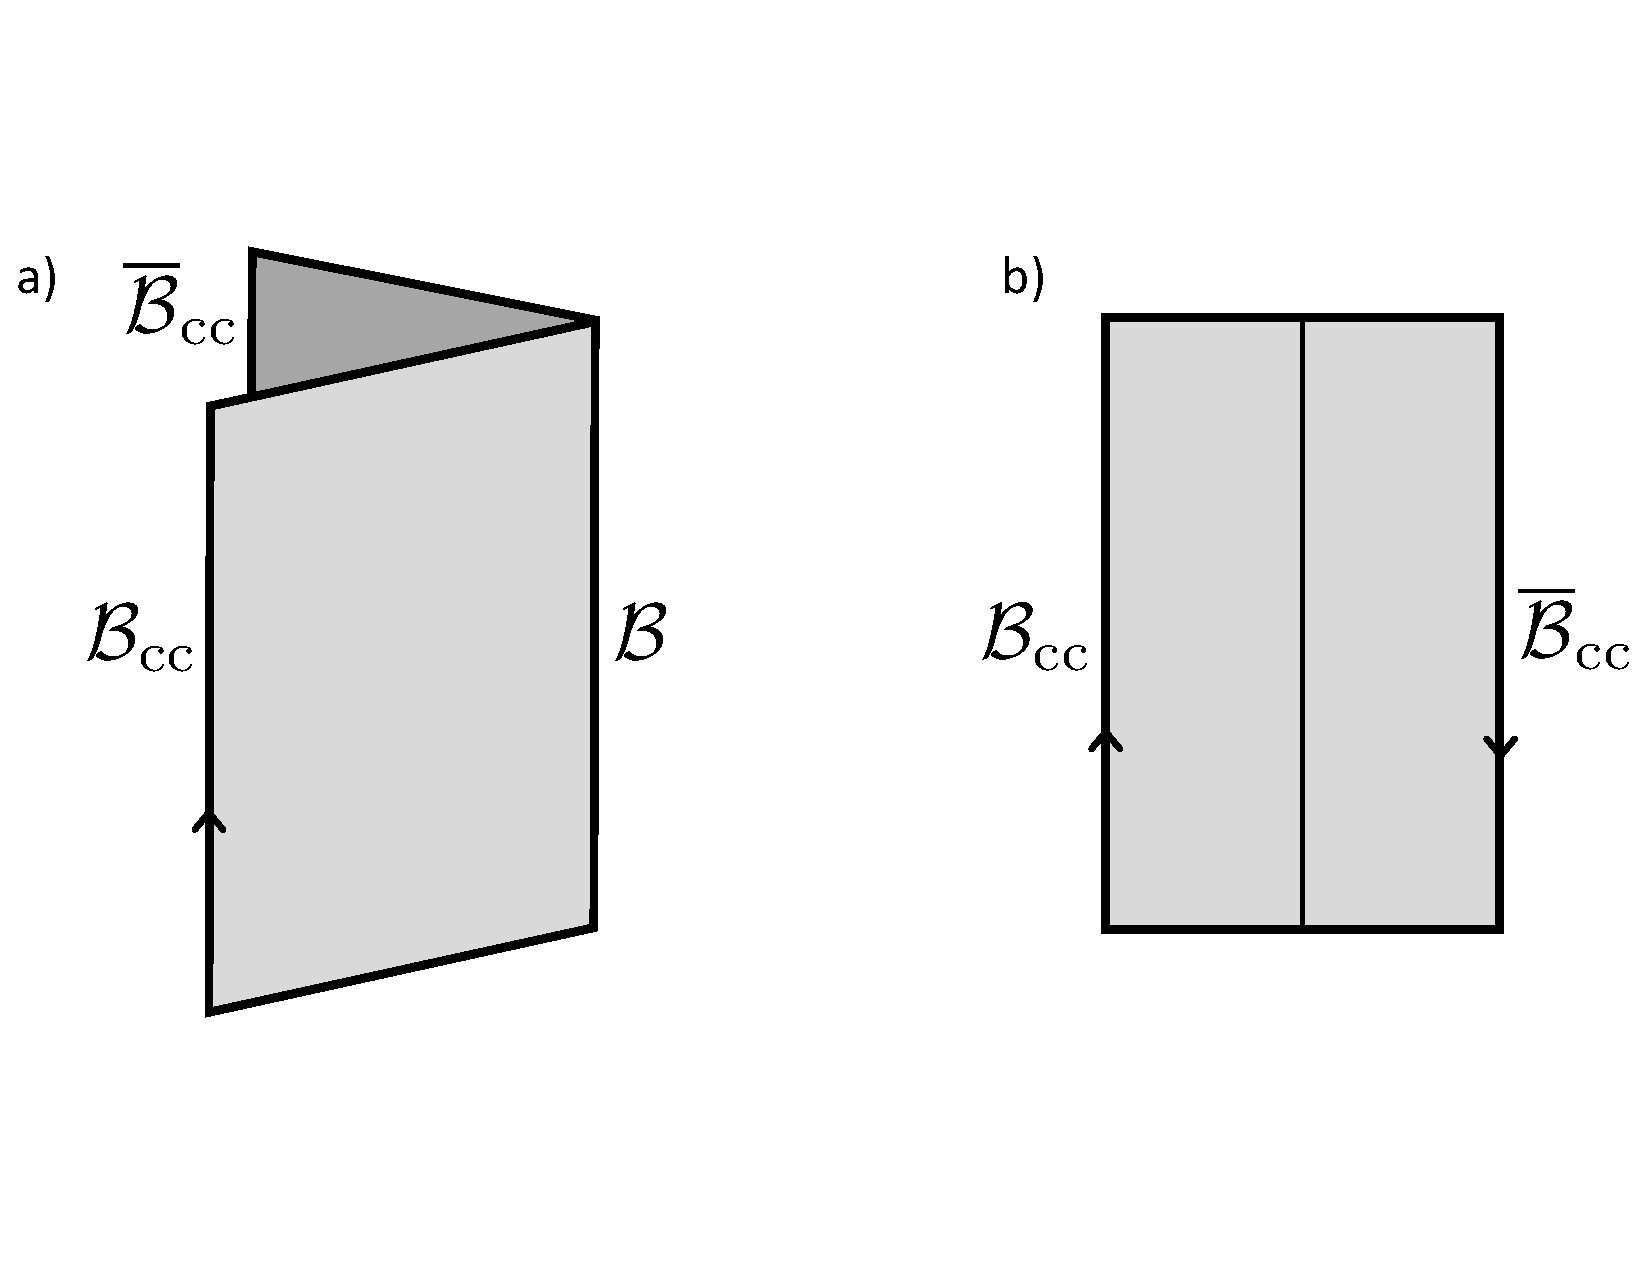
\includegraphics[width=4in]{Folding.pdf}
\end{center}
\caption{\small (a) 在折叠构造中，带状区域上有两份 $\sigma$-模型。除在右边界上由支撑于 $\h Y=Y_1\times Y_2$ 中对角线的膜 $\B$ 把它们粘合起来之外，这两个拷贝是解耦的。$\B$ 的 $\CP$ 丛平凡，因此这种粘合是它唯一的作用。(b) 展开之后，我们得到单个 $\sigma$-模型的拷贝，位于宽度加倍的带状区域上。$\B$ 的痕迹不再存在。\label{folding}}
\end{figure}

不过，这个定义有一个有用的变体。为计算 $\Hom(\B,\h\B_\cc)$，我们研究靶空间为 $\h Y$ 的 $\sigma$-模型，定义在带状区域 $\Sigma$ 上，左边界由 $\h\B_\cc$ 设定边界条件，右边界由 $\B$ 设定，如图 \ref{folding}(a)。$\h Y=Y_1\times Y_2$ 的两个因子在 $\sigma$-模型的体内解耦，因为 $\h Y$ 上的度量是乘积度量；它们在左边界上也解耦，因为膜 $\h\B_\cc=\B_{\cc,1}\times \B_{\cc,2}$ 同样是乘积。因此，在带状区域右边界之外，我们可以把 $\Sigma$ 看作有两叶，一叶映到 $Y_1$，一叶映到 $Y_2$，如图所示。两叶只在右边界上耦合；在那里，由于 $\B$ 支撑在 $Y_1\times Y_2$ 的对角线上，两叶被“粘在一起”，映到 $Y$ 中的同一点。这提示我们应该“展开”这幅图（图 \ref{folding}(b)）。展开之后，我们简单地得到宽度加倍的单叶，它映到 $Y$ 的单个拷贝。展开会反转折叠图中两叶之一的定向，而这种定向反转改变 $A$-模型辛形式的符号。在折叠图中，$A$-模型辛形式在 $Y_1$ 上是 $\frac{1}{2}\omega_K$，在 $Y_2$ 上是 $-\frac{1}{2}\omega_K$；因此展开之后，$A$-模型辛形式处处是 $\frac{1}{2}\omega_K$。换言之，展开图涉及 $Y$ 单个拷贝的通常 $A$-模型，其辛形式为 $\frac{1}{2}\omega_K$。展开之前，膜 $\B_{\cc,1}$ 与 $\B_{\cc,2}$ 的 $\CP$ 丛曲率都是 $\frac{1}{2} \omega_J$。反转 $\Sigma$ 的定向会把膜的 $\CP$ 丛换成其对偶丛（秩 1 情形下即其逆丛），从而反转 $\CP$ 曲率的符号。因此在展开图中，边界由膜 $\B_\cc$ 与 $\bB_\cc$ 标记，它们的 $\CP$ 丛分别是曲率为 $\frac{1}{2}\omega_J$ 与 $-\frac{1}{2}\omega_J$ 的线丛 $\L$ 与 $\L^{-1}$。\zy{原文作“lines bundles”，显系“line bundles”（线丛）之误；译文径改。} 这些就是第 \ref{background} 节引入的共轭典范余迷向膜。预量子线丛仍是 $\frL=\L^2$。$\A=\Hom(\B_\cc,\B_\cc)$ 是 $Y$ 上全纯函数交换代数 $\A_0$ 的形变量子化，$\b\A=\Hom(\bB_\cc,\bB_\cc)$ 类似地是 $Y$ 上反全纯函数代数 $\bA_0$ 的形变量子化。折叠图中的 $\H=\Hom(\B,\h\B_\cc)$，在展开图中变为 $\H=\Hom(\bar\B_\cc,\B_\cc)$。

无论用哪种描述 $\H$，我们都需要在 $\H$ 上定义埃尔米特内积。为确定起见，我们使用折叠的语言。\footnote{关于以下内容的更多细节，见 \cite{GW} 第 2.7 节。} 拓扑场论一般会给出 $\H=\Hom(\B,\h\B_\cc)$ 与其对偶空间 $\H'=\Hom(\h\B_\cc,\B)$ 之间的非退化双线性（而非埃尔米特）配对 $(~,~)$。要在 $\H$ 上得到埃尔米特配对，我们需要把这个双线性配对与一个从 $\H$ 到 $\H'$ 的反线性映射复合。在底层物理理论中，这样的映射由 $\sf{CPT}$ 对称性 $\Theta$ 提供。但 $\Theta$ 不是 $A$-模型对称性；它把 $A$-模型映到辛形式符号相反的共轭 $A$-模型。交换 $\h Y$ 两个因子的对合 $\tau$ 也把 $A$-模型与其共轭互换，因为它是反辛的（它反转 $A$-模型辛形式的符号），所以 $\Theta_\tau=\Theta\tau$ 是 $A$-模型的反线性对称性。最后，由于膜 $\B$ 与 $\B_\cc$ 是 $\Theta_\tau$-不变的，$\Theta_\tau$ 把 $\H$ 映到 $\H'$，于是我们可以通过
\be\label{hermdef}\la \psi,\psi'\ra= (\Theta_\tau\psi,\psi').\ee
在 $\H$ 上定义一个非退化埃尔米特配对。对一般的 $\Theta_\tau$-不变膜，这样的配对不是正定的。对于量子化余切丛这一特殊情形——它是我们在 $A$-模型一侧的主要例子——人们预期正定性成立。这一构造的 $B$-模型类比使用反全纯（而非反辛）对合 $\tau$。此情形下配对的正定性是微妙的，附录 \ref{bmodel} 中有讨论。

在折叠图中，$\tau$（因而 $\Theta_\tau$）交换 $\h Y=Y_1\times Y_2$ 的两个因子；在展开图中，它们交换带状区域的两端。交换带状区域的两端会反转带状区域的定向，从而会改变 $\sB$ 的符号。因此在 $\sB\not=0$ 的描述中，内积的定义不那么自然（需要给 $\Theta_\tau$ 配上一个 $B$-场规范变换）。这就是为什么我们在求解秩 1 余迷向膜的 Kapustin–Orlov 条件时取 $\sB=0$。
